\documentclass[a4paper,12pt]{article}
\usepackage[T1,T2A]{fontenc}
\usepackage[utf8]{inputenc}
\usepackage[english,ukrainian]{babel}


\usepackage{ upgreek }
\usepackage{amsmath}

\DeclareMathOperator*{\argmax}{arg\,max}
\DeclareMathOperator*{\argmin}{arg\,min}

\usepackage{graphicx}
\graphicspath{{./pictures/}}


\usepackage[unicode=true,colorlinks=true,urlcolor=blue,citecolor=green,linkcolor=blue]{hyperref}
\usepackage[ukrainian,nameinlink]{cleveref}
\usepackage{geometry} % Меняем поля страницы
\geometry{left=2cm}% левое поле
\geometry{right=1.5cm}% правое поле
\geometry{top=1cm}% верхнее поле
\geometry{bottom=2cm}% нижнее поле



\begin{document}
	
	\begin{titlepage}
		\vspace*{6cm}
		\begin{center}
			
			\large
			\textbf{Звіт}\\
			\textbf{до лабораторної роботи №4:}\\
			\textbf{<<Багатовимірна класифікація>>}
			
		\end{center}
		
		\vspace{8cm}
		\begin{flushright}
			студента 1-го курсу магістратури\\
			факультету комп'ютерних наук та кібернетики\\
			Кравця Олексія
		\end{flushright}
		
	\end{titlepage}

\newpage
\tableofcontents
\newpage
%document here
\section{Постановка задачі}

Маємо навчальну вибірку у вигляді векторів багатовимірного простору. Вибірка розподілена на 3 класи, що не перетинаються.

Необхідно, на базі навчальної вибірки, провести класифікацію тестової вибірки трьома різними методами.

\section{Опис методів}

Для класифікації використовуються центри мас класів

\begin{displaymath}
	M_k =\frac{\sum_{j=1}^L \textbf{y}^k_j}{L}
\end{displaymath}

де $M_k$ -- центр мас $k$-го класу, $L$ -- кількість елементів (векторів) у класі, $y_j^k$ -- елемент (вектор) $k$-го класу.

Нехай $M^1, \ldots, M^m$ -- центи мас класів. $X = \left( x_1, \ldots, x_n \right)$ -- точка, яку необхідно класифікувати.

\subsection{Метод 1}

Будемо класифікувати точки за найбільш суттєвою різницею до центрів мас класів. Тобто для кожного виміру $i \in \{1,2,\ldots, n \}$ будемо рахувати відстань від точки до центрів мас класів та рахувати наступний вираз для кожного класу

\begin{equation}
	\frac{|M^k_i -x_i|}{ \left(\sum_{j \ne k} |M^j_i - x_i|\right)/(m-1)}
\end{equation}
ділимо відстань до поточного класу на середню відстань до інших класів. Або

\begin{equation} \label{eq_min}
	\frac{|M^k_i -x_i|}{\min_{j \ne k} |M^j_i - x_i|}
\end{equation}
ділимо відстань до поточного класу на мінімальну відстань до інших класів.

В результаті отримуємо $m \cdot n$ значень (для кожного виміру та кожного класу). Вибираємо мінімальне значення, і клас, що йому відповідає, буде результатом.

\subsection{Метод 2}

Для класифікації точки обираємо той клас, що має найменшу відстань о точки по найбільшій кількості вимірів. Отже, рахуємо наступний вираз

\begin{equation}
	\left( \argmin_{j \in\{1,\ldots, m\}}|M^j_1 - x_1|, \ldots, \argmin_{j \in \{1,\ldots, m\}}|M^j_n - x_n| \right)
\end{equation}

І вибираємо той клас, що зустрівся більше всіх.

\subsection{Метод 3}

Порахуємо суму відстаней від точки до центрів мас класів по кожному виміру. Оберемо той клас, у якого сумма найменша. Отже, обираємо клас за наступним правилом
\begin{equation}
	\argmin_{j \in \{1,\ldots, m\}} \left( \sum_{i=1}^n |M_i^j - x_i| \right)
\end{equation}


\section{Результати}

\subsection{Тести на площині}

Для наочності провели класифікацію точок на площині. У \textbf{Методі 1} було використано рівняння (\ref{eq_min}).


\begin{figure}[h]
	\begin{minipage}[h]{0.5\linewidth}
		\center{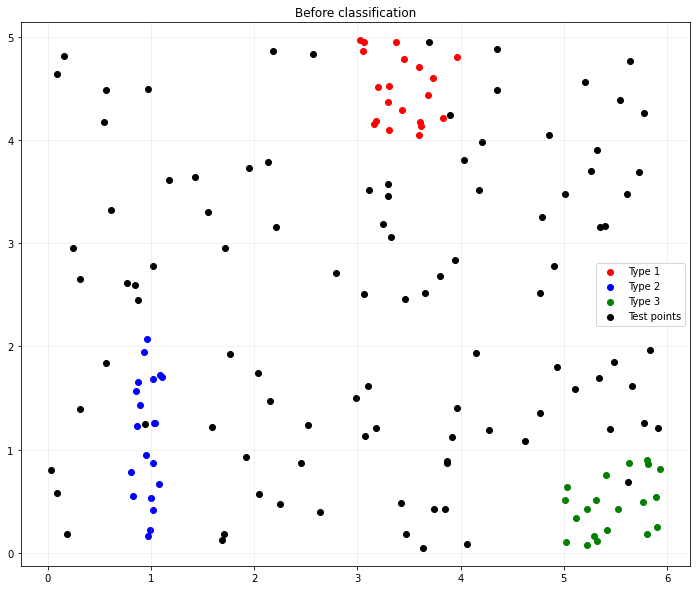
\includegraphics[width=1\linewidth]{fig1.png}} \\
	\end{minipage}
	\hfill
	\begin{minipage}[h]{0.47\linewidth}
		\center{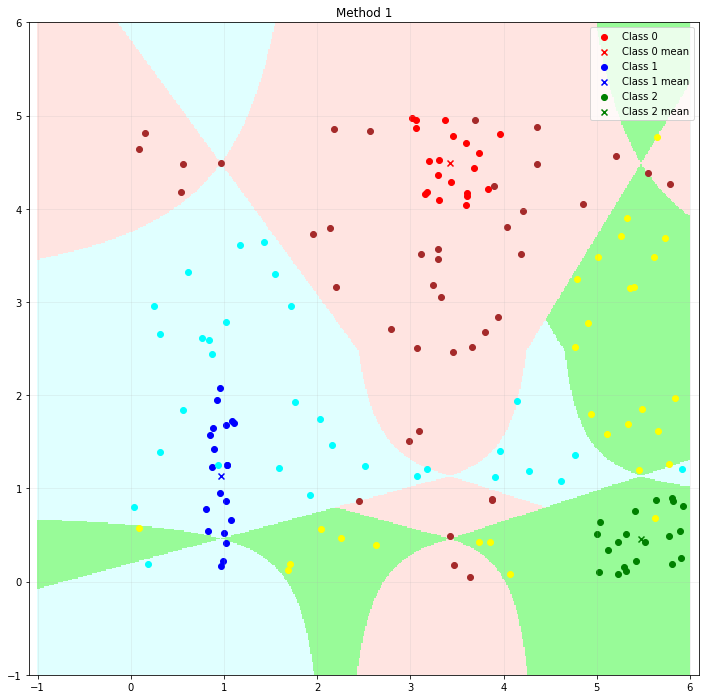
\includegraphics[width=1\linewidth]{fig2.png}} \\
	\end{minipage}
	\vfill
	\begin{minipage}[h]{0.47\linewidth}
		\center{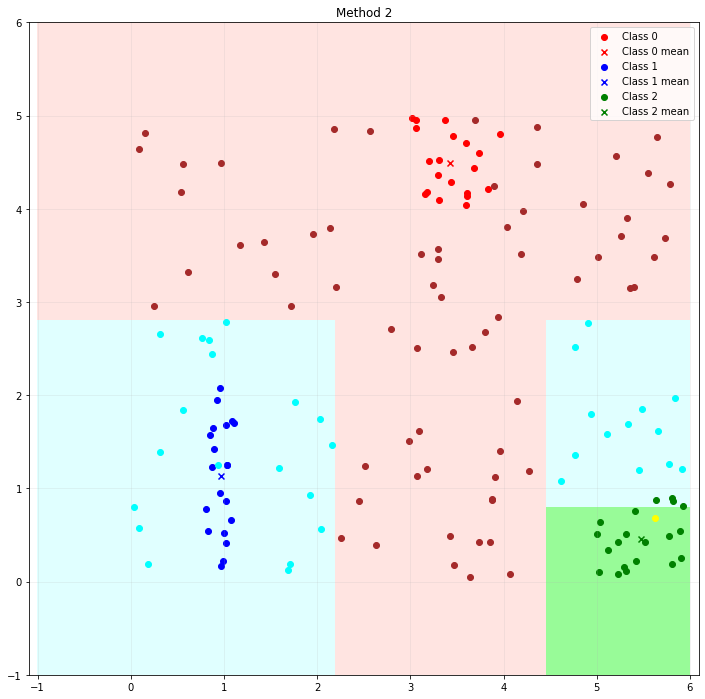
\includegraphics[width=1\linewidth]{fig3.png}} \\
	\end{minipage}
	\hfill
	\begin{minipage}[h]{0.47\linewidth}
		\center{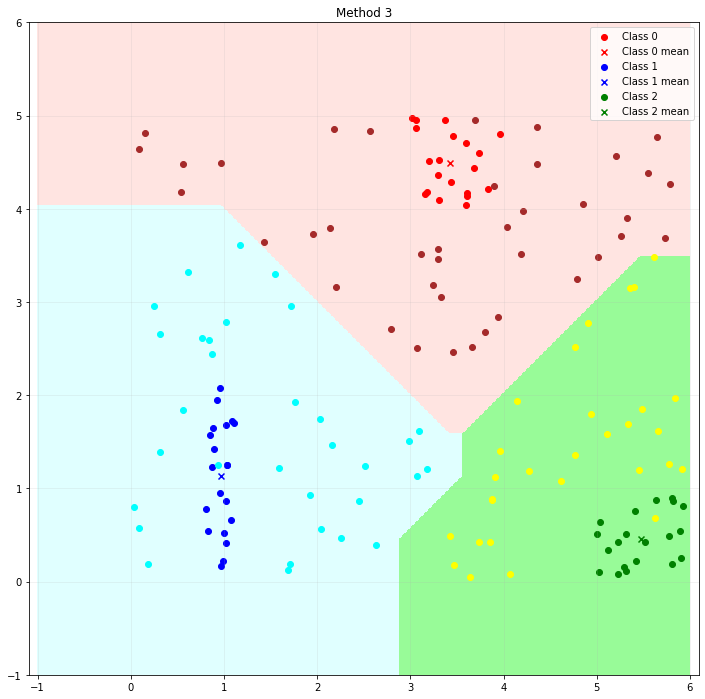
\includegraphics[width=1\linewidth]{fig4.png}} \\
	\end{minipage}
	\caption{}
	\label{ris:experimentalcorrelationsignals}
\end{figure}

Якщо розглянути результати більш детально, то можна помітити, що \textbf{Метод 2} не може точно класифікувати багато точок. Розглянемо перші $10$ тестових точок

\begin{verbatim}
Dot: [5.65745822 1.61601466] has class: [1, 2]
Dot: [3.11274373 3.51509479] has class: [0]
Dot: [2.18177761 4.85891041] has class: [0, 1]
Dot: [5.77468377 1.25891148] has class: [1, 2]
Dot: [2.98349104 1.50439155] has class: [0, 1]
Dot: [1.70904297 0.18443474] has class: [1, 2]
Dot: [3.657386   2.51339512] has class: [0, 1]
Dot: [0.30887251 1.39323232] has class: [1]
Dot: [5.44959532 1.19780945] has class: [1, 2]
Dot: [0.86936923 2.4472638 ] has class: [1]
\end{verbatim}

Легко помітити, що \textbf{Метод 2} не може класифікувати деякі точки.

\subsection{Багатовимірна класифікація}

Для тестування багатовимірної класифікації я обрав набір даних <<Іриси Фішера>>. Кожний елемент набору даних це -- чотиривимірний вектор, що розподілений в один з трьох класів. Точність класифікації я оцінюю так

\begin{displaymath}
	\text{точність}=\frac{\text{кількість правильних класифікацій}}{\text{загальна кількість класифікацій}}
\end{displaymath}

Також будемо проводити крос-валідацію. Розділимо набір даних на $5$ частин. 

Виведемо таблицю з отриманою точністю. 

\begin{tabular}{| l | c | c | c | c | c | c |}
	\hline
	Метод & \textit{fold 1} & \textit{fold 2} & \textit{fold 3} & \textit{fold 4} & \textit{fold 5} & mean \\
	\hline
	
	\textbf{Метод 1} \textit{min} & $0.867$&  $0.867$& $0.733$ & $0.9$ &  $0.8$& $0.833$ \\
	
	\textbf{Метод 1} \textit{mean} & $0.9$ & $0.867$ & 
	$0.767$ & $0.933$ & $0.833$ & $0.86$ \\
	
	\textbf{Метод 2} & $0.933$ & $0.9$ & $0.933$ & $0.967$ & $0.833$ & $0.913$ \\
	\textbf{Метод 3} & $0.967$& $0.9$ &$0.8$ & $0.967$& $0.8$ & $0.887$\\
	\hline
\end{tabular}

\section{Висновок}
	\textbf{Метод 2} показав найкращі результати на Ірисах Фішера, однак для класифікації точок на площині цей метод показує себе погано. Він не може класифікувати деякі точки.
\end{document}
